\section{GObject}\label{gobject}

\subsection{Class and instance}\label{class-and-instance}

GObject instance is created with
\passthrough{\lstinline!g\_object\_new!} function. GObject has not only
instances but also classes.

\begin{itemize}
\tightlist
\item
  A class of GObject is created at the first call of
  \passthrough{\lstinline!g\_object\_new!}. And there exists only one
  GObject class.
\item
  GObject instance is created whenever
  \passthrough{\lstinline!g\_object\_new!} is called. So, two or more
  GObject instances can exist.
\end{itemize}

In a broad sense, GObject means the object which includes its class and
instances. In a narrow sense, GObject is a definition of a C structure.

\begin{lstlisting}[language=C]
typedef struct _GObject  GObject;
struct  _GObject
{
  GTypeInstance  g_type_instance;
  
  /*< private >*/
  guint          ref_count;  /* (atomic) */
  GData         *qdata;
};
\end{lstlisting}

The \passthrough{\lstinline!g\_object\_new!} function allocates
GObject-sized memory, initializes the memory and returns the pointer to
the memory. The memory is a GObject instance.

In the same way, the class of GObject is memory allocated by
\passthrough{\lstinline!g\_object\_new!} and its structure is defined
with GObjectClass. The following is extracted from
\passthrough{\lstinline!gobject.h!}. But you don't need to know the
details of the structure now.

\begin{lstlisting}[language=C]
struct  _GObjectClass
{
  GTypeClass   g_type_class;

  /*< private >*/
  GSList      *construct_properties;

  /*< public >*/
  /* seldom overridden */
  GObject*   (*constructor)     (GType                  type,
                                 guint                  n_construct_properties,
                                 GObjectConstructParam *construct_properties);
  /* overridable methods */
  void       (*set_property)        (GObject        *object,
                                         guint           property_id,
                                         const GValue   *value,
                                         GParamSpec     *pspec);
  void       (*get_property)        (GObject        *object,
                                         guint           property_id,
                                         GValue         *value,
                                         GParamSpec     *pspec);
  void       (*dispose)         (GObject        *object);
  void       (*finalize)        (GObject        *object);
  /* seldom overridden */
  void       (*dispatch_properties_changed) (GObject      *object,
                         guint     n_pspecs,
                         GParamSpec  **pspecs);
  /* signals */
  void       (*notify)          (GObject    *object,
                     GParamSpec *pspec);

  /* called when done constructing */
  void       (*constructed)     (GObject    *object);

  /*< private >*/
  gsize     flags;

  gsize         n_construct_properties;

  gpointer pspecs;
  gsize n_pspecs;

  /* padding */
  gpointer  pdummy[3];
};
\end{lstlisting}

The programs for GObject are included in GLib source files. You can
download the GLib source files from
\href{https://download.gnome.org/sources/glib/}{GNOME download page}.

There are sample programs in src/misc directory in the GObject tutorial
repository. You can compile them by:

\begin{lstlisting}
$ cd src/misc
$ meson setup _build
$ ninja -C _build
\end{lstlisting}

One of the programs is \passthrough{\lstinline!example1.c!}. Its code is
as follows.

\begin{lstlisting}[language=C, numbers=left]
#include <glib-object.h>

int
main (void)
{
  GObject *instance1 = g_object_new (G_TYPE_OBJECT, NULL);
  GObject *instance2 = g_object_new (G_TYPE_OBJECT, NULL);
  g_print ("The address of instance1 is %p\n", instance1);
  g_print ("The address of instance2 is %p\n", instance2);

  GObjectClass *class1 = G_OBJECT_GET_CLASS (instance1);
  GObjectClass *class2 = G_OBJECT_GET_CLASS (instance2);

  g_print ("The address of the class of instance1 is %p\n", class1);
  g_print ("The address of the class of instance2 is %p\n", class2);
  g_print ("Class Name: %s\n", G_OBJECT_CLASS_NAME (class1));

  g_object_unref (instance1);
  g_object_unref (instance2);
}
\end{lstlisting}

\begin{itemize}
\tightlist
\item
  5-6: \passthrough{\lstinline!instance1!} and
  \passthrough{\lstinline!instance2!} are pointers that points GObject
  instances. \passthrough{\lstinline!class1!} and
  \passthrough{\lstinline!class2!} points a class of the instances.
\item
  8-11: A function \passthrough{\lstinline!g\_object\_new!} creates a
  GObject instance. GObject instance is a chunk of memory which has
  GObject structure (\passthrough{\lstinline!struct \_GObject!}). The
  argument \passthrough{\lstinline!G\_TYPE\_OBJECT!} is the type of
  GObject. This type is different from C language type like
  \passthrough{\lstinline!char!} or \passthrough{\lstinline!int!}. There
  is \emph{Type System} which is a base system of GObject system. Every
  data type such as GObject must be registered to the type system. The
  type system has series of functions for the registration. If one of
  the functions is called, then the type system determines
  \passthrough{\lstinline!GType!} type value for the object and returns
  it to the caller. \passthrough{\lstinline!GType!} is an unsigned long
  integer on my computer but it depends on the hardware.
  \passthrough{\lstinline!g\_object\_new!} allocates GObject-sized
  memory and returns the pointer to the top address of the memory. After
  the creation, this program displays the addresses of instances.
\item
  13-16: A macro \passthrough{\lstinline!G\_OBJECT\_GET\_CLASS!} returns
  the pointer to the class of the argument. Therefore,
  \passthrough{\lstinline!class1!} points the class of
  \passthrough{\lstinline!instance1!} and
  \passthrough{\lstinline!class2!} points the class of
  \passthrough{\lstinline!instance2!} respectively. The addresses of the
  two classes are displayed.
\item
  18-19: \passthrough{\lstinline!g\_object\_unref!} will be explained in
  the next subsection. It destroys the instances and the memory is
  freed.
\end{itemize}

Now, execute it.

\begin{lstlisting}
$ cd src/misc; _build/example1
The address of instance1 is 0x55895eaf7ad0
The address of instance2 is 0x55895eaf7af0
The address of the class of instance1 is 0x55895eaf7880
The address of the class of instance2 is 0x55895eaf7880
\end{lstlisting}

The locations of two instances \passthrough{\lstinline!instance1!} and
\passthrough{\lstinline!instance2!} are different. Each instance has its
own memory. The locations of two classes
\passthrough{\lstinline!class1!} and \passthrough{\lstinline!class2!}
are the same. Two GObject instances share the same class.

\begin{figure}
\centering
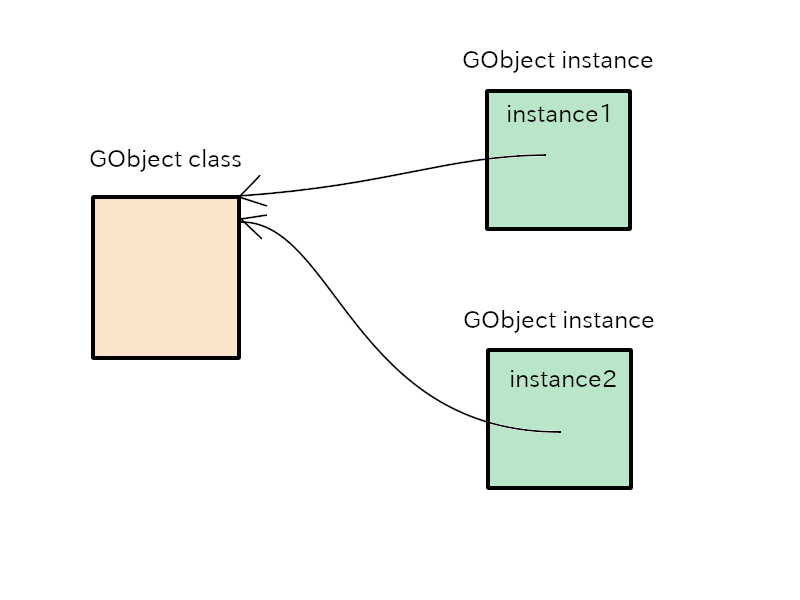
\includegraphics[width=10cm,height=7.5cm]{../image/class_instance.png}
\caption{Class and Instance}
\end{figure}

\subsection{Reference count}\label{reference-count}

GObject instance has its own memory. They are allocated by the system
when it is created. If it becomes useless, the memory must be freed.
However, how can we determine whether it is useless? GObject system
provides reference count to solve the problem.

An instance is created and used by other instance or the main program.
That is to say, the instance is referred. If the instance is referred by
A and B, then the number of the reference is two. This number is called
\emph{reference count}. Let's think about a scenario like this:

\begin{itemize}
\tightlist
\item
  A calls \passthrough{\lstinline!g\_object\_new!} and owns an instance
  G. A refers G, so the reference count of G is 1.
\item
  B wants to use G too. B calls \passthrough{\lstinline!g\_object\_ref!}
  and increases the reference count by 1. Now the reference count is 2.
\item
  A no longer uses G. A calls \passthrough{\lstinline!g\_object\_unref!}
  and decreases the reference count by 1. Now the reference count is 1.
\item
  B no longer uses G. B calls \passthrough{\lstinline!g\_object\_unref!}
  and decreases the reference count by 1. Now the reference count is 0.
\item
  Because the reference count is zero, G knows that no one refers to it.
  G begins finalizing process by itself. G disappears and the memory is
  freed.
\end{itemize}

A program \passthrough{\lstinline!example2.c!} is based on the scenario
above.

\begin{lstlisting}[language=C, numbers=left]
#include <glib-object.h>

static void
show_ref_count (GObject *instance)
{
  if (G_IS_OBJECT (instance))
    {
      g_print ("Reference count is %d.\n", instance->ref_count);
    }
  else
    {
      g_print ("Instance is not a GObject.\n");
    }
}

int
main (void)
{
  GObject *instance = g_object_new (G_TYPE_OBJECT, NULL);
  g_print ("Call g_object_new.\n");
  show_ref_count (instance);
  g_object_ref (instance);
  g_print ("Call g_object_ref.\n");
  show_ref_count (instance);
  g_object_unref (instance);
  g_print ("Call g_object_unref.\n");
  show_ref_count (instance);
  g_object_unref (instance);

  g_print ("Call g_object_unref.\n");
  g_print ("Now the reference count is zero and the instance is destroyed.\n");
  g_print ("The instance memories are possibly returned to the system.\n");
  g_print ("Therefore, the access to the same address may cause a segmentation error.\n");
}
\end{lstlisting}

Now execute it.

\begin{lstlisting}
$ cd src/misc; _build/example2
bash: cd: src/misc: No such file or directory
Call g_object_new.
Reference count is 1.
Call g_object_ref.
Reference count is 2.
Call g_object_unref.
Reference count is 1.
Call g_object_unref.
Now the reference count is zero and the instance is destroyed.
The instance memories are possibly returned to the system.
Therefore, the access to the same address may cause a segmentation error.
\end{lstlisting}

\passthrough{\lstinline!example2!} shows:

\begin{itemize}
\tightlist
\item
  \passthrough{\lstinline!g\_object\_new!} creates a new GObject
  instance and sets its reference count to 1.
\item
  \passthrough{\lstinline!g\_object\_ref!} increases the reference count
  by 1.
\item
  \passthrough{\lstinline!g\_object\_unref!} decreases the reference
  count by 1. If the reference count drops to zero, the instance
  destroys itself.
\end{itemize}

\subsection{Initialization and destruction
process}\label{initialization-and-destruction-process}

The actual process of GObject initialization and destruction is very
complex. The following is simplified description without details.

Initialization

\begin{enumerate}
\def\labelenumi{\arabic{enumi}.}
\tightlist
\item
  Registers GObject type with the type system. This is done in the GLib
  initialization process before the function
  \passthrough{\lstinline!main!} is called. (If the compiler is gcc,
  then \passthrough{\lstinline!\_\_attribute\_\_ ((constructor))!} is
  used to qualify the initialization function. Refer to
  \href{https://gcc.gnu.org/onlinedocs/gcc-10.2.0/gcc/Common-Function-Attributes.html\#Common-Function-Attributes}{GCC
  manual}.)
\item
  Allocates memory for GObjectClass and GObject structure.
\item
  Initializes the GObjectClass structure memory. This memory will be the
  class of GObject.
\item
  Initializes the GObject structure memory. This memory will be the
  instance of GObject.
\end{enumerate}

This initialization process is carried out when
\passthrough{\lstinline!g\_object\_new!} function is called for the
first time. At the second and subsequent call for
\passthrough{\lstinline!g\_object\_new!}, it performs only two
processes: (1) memory allocation for GObject structure (2)
initialization for the memory. \passthrough{\lstinline!g\_object\_new!}
returns the pointer that points the instance (the memory allocated for
the GObject structure).

Destruction

\begin{enumerate}
\def\labelenumi{\arabic{enumi}.}
\tightlist
\item
  Destroys GObject instance. The memory for the instance is freed.
\end{enumerate}

GObject type is a static type. Static type never destroys its class. So,
even if the destroyed instance is the last instance, the class still
remains.

When you write code to define a child object of GObject, It is important
to understand the process above. The detailed process will be explained
in the later sections.
